\documentclass[../tfm.tex]{subfiles}
\begin{document}
\textit{Aportar detalles del proceso de desarrollo incluyendo fases e hitos del proceso, diagramas representativos de la arquitectura y funcionamiento, capturas de pantalla para ilustrar el funcionamiento, etc.}

El desafío de consolidar en un sistema portable una aplicación autónoma de detección de caídas debe hacer frente a una serie de limitaciones.

\section{Desafíos}

El objetivo de todo modelo de detección de eventos es lograr un sistema que consiga capturar la totalidad de las realizaciones del mismo con el menos número posible de falsos positivos. En otras palabras, buscamos un sistema con una especificidad y sensibilidad de 100\%\cite{Noury2007}. \todo{Añadir referencias a papers, comentarios sobre sensibilidad y especificidad}.

\subsection{Usabilidad}
El primer reto de toda aplicación es conseguir una experiencia de usuario adaptada al cliente final. De nada sirve lograr implementar una plataforma que cumpla perfectamente con todos los requisitos y objetivos funcionales si el producto resultante se utiliza.

\subsubsection{Público objetivo}
Como se ha mencionado en la introducción del trabajo, los daños relacionados con las caídas son una de las principales causas de mortaldad entre las personas mayores de 65 años \todo{cita requerida}. Es propio de este grupo de población la desafección por la tecnología y la carencia o desinterés por su uso. Esta condición ha de ser tenida en cuenta para el desarrollo de cualquier producto.

Las personas de edad avanzada suelen padecer así mismo de otras condiciones que pueden limitar su grado de movilidad, atención o memoria que impidan o reduzcan la posibilidad de adaptarse o incorporar nuevas rutinas. Los problemas motores y de percepción reducen notablemente la capacidad de mostrar información así como de interactuar con el usuario cuando se necesite una acción por su parte.

Se entiende por tanto que si se ha de realizar un producto para esta población, es requisito que sea lo menos obtrusivo posible, siendo recomendable incorporar la funcionalidad a un objeto de uso cotidiano para evitar la modificación de rutinas o la reticencia a incorporar nuevos procesos o elementos en su vida diaría. La interfaz de usuario debe ser mínima, usando un lenguaje visual que resulte familiar alejado de los estándares de las aplicaciones modernas. Así mismo, reducir o eliminar los procesos de configuración y manipulación, con un sistema que funcione al salir de la caja \todo{mala traducción de \textit{out of the box}}.

\subsubsection{Localización}

Una de las decisiones con mayor impacto sobre la funcionalidad del prototipo es la elección de la posición del dispositivo de captura ya que influencia en gran medida a la capacidad de detección de caídas \cite{Kangas2008}. Diversos estudios muestran que el mejor lugar para posicionar un sistema de medición de la aceleración para detectar caídas es la cintura, seguida de la cabeza siendo posible también usar un medidor en la muñeca\cite{Chen2005, Kangas2008, Noury2007}. Si bien estos resultados se basan en el análisis de métodos analíticos basados en cotas, se desprende de ellos la actitud o posición del cuerpo es un buen indicador para la predicción de actividades, razón por la que realizar la captura en muñecas o tobillos, las extremidades más alejadas del tronco, sufren de mayores penalizaciones para conseguir buenas estimaciones.

Al optarse por un reloj o \textit{pulsera de actividad} como plataforma para la implementación las opciones para posicionar la unidad de medida quedan reducida a una: la muñeca.

\subsection{Conectividad}

Hasta la fecha, los sistemas de detección de caídas se basan en arquitecturas cliente servidor para disociar el módulo de cómputo del de captura y conseguir que el dispositivo a llevar en si sea del menor tamaño posible. Este acercamiento que permite solventar el problema que derivaría de tener que llevar un obtrusivo sistema sobre si añade el problema de la necesidad de un enlace o comunicación con el módulo de cálculo. Ganamos en usabilidad pero perdemos en portabilidad.\todo{Cita y referencias a sistemas comerciales}

El principal problema de la conectividad radica en el hecho de que a pérdida de comunicación entre ambos módulos deriva en un sistema con ninguna capacidad. El módulo de cálculo, privado de datos no es capaz de realizar ninguna detección. Por su parte el aparato de captura, por si mismo, no tiene capacidad alguna para realizar nada más que la lectura.

El sistema implementado opta por una arquitectura cliente-pesado y servidor ligero. El cliente tiene suficiente capacidad para realizar captura, cómputo y capacidad de alerta como para funcionar de forma aislada. El servidor realiza funciones de expansión de la capacidad de alerta de la plataforma, así como de distribución de actualizaciones o mejoras en modelos y parámetros, pero de ninguna manera resulta imprescindible para el funcionamiento del dispositivo portable. Este es el principio básico y director de este trabajo: implementar una plataforma autónoma de detección de caídas capaz de ejecutarse en un dispositibo llevable.

\subsection{Rendimiento}

Como en toda imlpementación, el

\section{Plataforma}

Para el servidor optamos por una arquitectura de microservicios usando la plataforma de AWS Lambda con almacenamiento en S3

Para el dispositivo móvil usamos un reloj inteligente Fossil Sport con sistema operativo WearOS y por tanto compatible con el ecosistema Android.

El la generación, entrenamiento, análisis y evaluación de modelos se realiza usando Keras/Tensorflow corriendo en la plataforma Google Colab.

\section{Arquitectura}

\subsection{Arquitectura del sistema}

\subsection{Arquitectura de la aplicación}

El sistema está compuesto por dos bloques funcionales tal y como se muestra en \ref{fig:clasesUml}. Tenemos un bloque o paquete que incluye los servicios encargados del registro de datos de los sensores, gestión de entradas y notificación de eventos, implementación del algoritmo de detección y comunicación con el servidor. Este primer bloque contiene a su vez una aplicación de gestión del servicio que permite realizar tareas de mantenimiento y configuración. En un segundo bloque tenemos la interfaz del usuario principal, encargada de lanzar la aplicación, alertar en caso de caída y capturar la respuesta del usuario en caso de necesitarla.

\figura{classUML}{fig:clasesUml}{Diagrama de clases de la aplicación}

Desde el punto de vista del usuario la aplicación provée dos puntos de entrada. La interfaz principal toma la forma de una \textit{watchface}. En \textit{WearOS}, una \textit{watchface} se corresponde con un tipo específico de aplicación que realiza principalmente la función de mostrar la hora al usuario. Realiza la función de "escritorio" del sistema y es por tanto el punto inicial de toda interacción del usuario con el sistema. Este acercamiento permite solventar dos problemas:

Facilita la experiencia de usuario al no requerir de ninguna acción por parte del usuario para poner en marcha la aplicación. Al convertirse en la aplicación principal del reloj con  \textit{WearOS} garantizamos que el propio sistema operativo lanzará en el arranque y mantendrá activa la actividad en todo momento.

La aplicación toma forma de un objeto cotidiano e interactúa con el usuario utilizando un concepto conocido para este: un reloj digital. La única información que se muestra al usuario es la hora (adicionalmente el propio sistema operativo sobreimprime indicaciones de batería baja, ausencia de conexión a internet y existencia de notificaciones de otros servicios y aplicaciones). De esta forma, para el usuario, el dispositivo se convierte en un objeto conocido con un uso muy extendido que de forma adicional a su función tradicional realiza el proceso de detección de caídas.

En esta aplicación se han reducido al máximo las interacciones requeridas por parte del usuario en todo momento, hasta el punto de no requerir ninguna. La aplicación funciona en todo momento com un reloj tradicional mostrando la hora de forma analógica mediante unas manecillas. En el caso de detectarse una caída o evento similar, emitirá de forma automática una serie de avisos visuales, acústicos y táctiles que podrán ser desactivados si se detecta actividad nuevamente. Aunque también existe la posibilidad de desactivarlos tocando la pantalla.

La segunda interfaz que provee la aplicación se encarga de las tareas de administración y configuración. Permite introducir un nombre del usuario y forzar el estado de funcionamiento de los servicios de captura y detección. Si bien ninguno de estos procesos es necesario, se ofrece para facilitar la puesta en marcha y prueba del sistema.

El proceso que contiene la lógica principal, descrita en la figura\ref{fig:deteccionFlow}, se encuentra en la clase \textit{AccelSensorRead}. Este servicio es lanzado automáticamente al ejecutarse cualquiera de las dos interfaces de usuario provistas, y se mantiene ejecutándose de fondo. Se encarga de:

\begin{itemize}
  \item Recupera configuración previa
  \item Configurar y leer las muestras del acelerómetro
  \item Realizar el primer proceso de detección (algoritmo basado en cotas)
  \item Lanzar el proceso de análisis usando el modelo ML y recuperar el resultado
  \item Alertar y notificar del evento tanto a los clientes locales como a los servidores remotos
\end{itemize}

El proceso de detección o filtrado usando el modelo implementado basado en redes recurrentes es el único que se exporta a una clase propia: \textit{CrashDetectService}. Toma de nuevo la forma de un servicio asíncrono que es invocado únicamente cuando el modelo analítico ha detectado un positivo. De esta forma se pretende reducir drásticamente las necesidades de cómputo. Este servicio a su vez se subdivide en unos módulos que son los modelos de detección propiamente dichos. Como se aprecia en el diagrama UML de la arquitectura\ref{fig:clasesUml}, es la clase \textit{TFLiteModelDetector} la que provee la cumunicación con el modelo de TFLite previamente generado y entrenado en Colab.

\section{Implementación}

\subsection{Algoritmo}

El algoritmo de detección consta de dos fases consecutivas, tal y como se muestra en el diagrama \ref{fig:deteccionFlow}. Un primer bloque usando un algoritmo analítico basado en la variación del vector suma de la acceleración y una posterior etapa de depuración o filtrado basado en un modelo de detección de anomalías usando RNN.

\figura{deteccionFlujo}{fig:deteccionFlow}{Flujo de trabajo de la aplicación de detección de caidas}

\subsubsection{Modelo Analítico}

Los modelos analíticos aplicados a la detección de caídas tienen la gran ventaja de ser computacionalmente simples. Su mayor contraprestación es la dificultad de balancear las métricas de Especificidad y Sensibilidad. Al basarse en niveles o cotas, podemos aumentar la sensibilidad situando el nivel de estas de manera que la sensibilidad llegue al 100\%, como requieren los algoritmos de Bourke\cite{Bourke2006}. Sin embargo esto afectará a la especificidad negativamente\cite{Aziz2017}.

\warn{Actualmente usa $SVTot_n - SVTot_{n-1} < 2G$ como algoritmo. Bourke en pruebas con 3.5G de límite. Sección a revisar}

En nuestro algoritmo general, el modelo analítico es similar a una capa de gestión de la atención del modelo RNN. Es por esta razón que la baja especificidad  no resulta un problema ya que lo que nos interesa es que esta etapa tenga una sensibilidad del 100\%. El dispositivo captura información de la aceleración en 3 ejes con una medida máxima de $9G$ y a una frecuencia de muestreo $f_m=50Hz$.

Como primera etapa se utiliza un algoritmo basado el el vecotor total de la aceleración ($SVTot = |\sqrt{a_{x}^2+a_{y}^2+a_{z}^2}|$) por su simplicidad de cálculo. En concreto, comparamos el valor absoluto de la diferencia de dos mediciones consecutivas de la aceleración y comparamos con un umbral de referencia.
\[
ModeloAnalitico\rightarrow |SVTot_n - SVTot_{n-1}|\geq A_{umbral}
\]

El valor de $A_{umbral}$ se obtiene experimentalmente gracias al análisis de los datos obtenidos. Se fija en $A_{umbral} = 3G$ que resulta un buen equilibrio ya que conseguimos una cantidad reducida de eventos manteniendo un nivel bajo\todo{citar trabajos y medidas. Bourke usa 3,5G, otros usan valores más altos, la mayoría de caídas tienen niveles instantáneos de SVTot superiores a 6G}.\todo{incluir trabajo estadístico de los datos de aceleración del dataset} \todo{incluir gráfica temporal explicativa del algoritmo}

Si se sobrepasa el umbral en $t=0$. El sistema envía instantáneamente al siguiente modelo las muestras entre $t=-225$ y $t=-25$ (4 segudnos previos al evento). En segundo plano sigue capturando muestras hasta $t=25$. Este segundo bloque de 50 muestras (un segundo centrado en el evento) se envía también a la siguiente etapa. La decisión de separar el envío de datos a la siguiente etapa está motivada por la reducción de la latencia del sistema y obtener una clasificación o resultado con la menor dilación posible.


\subsubsection{Modelo RNN}

El modelo RNN comporta a su vez dos bloques. Un primer bloque de predicción y un segundo de detección de anomalías.

\paragraph{Limitaciones de la plataforma}
Al ejecutarse sobre un intérprete de TFLite, el modelo implementado sufre las restricciones que esta plataforma impone. Las de mayor impacto a este proyecto es la del uso de celdas GRU, no soportadas de forma nativa\cite{tfliteGru}, de la misma forma que las redes RNN bidireccionales, que no pueden ser portadas directamente a a TFLite\cite{tfliteBidir} ni se les puede aplicar pruning para reducir su tamaño\cite{tfPruneBidir}. Este último problema tiene sin embargo una alternativa consistente en usar una capa personalizada que implemente la interfaz de pruning y consista en dos redes LSTM, una normal y otra regresiva.


\paragraph*{Predicción}
\info{Detalles del modelo pueden variar fácilmente. Actualmente usando LSTM bidireccional 50 unidades. }

\figura{modeloRNN}{fig:rnnModel}{Modelo RNN}

El modelo predictivo, se basa en la capacidad de las redes RNN y particularmente las basadas en celdas LSTM y GRU para generar modelos predictivos de calidad para series temporales de señales estacionarias \cite{Qin2019}.

La arquitectura el modelo usa una red LSTM bidireccional con 50 unidades de memoria y una única salida. Tal y como se observa en el diagrama \ref{fig:rnnModel} a partir de la primera serie de 200 muestras recibidas el modelo es capaz de generar la predicción de la muestra siguiente.

Para conseguir la predicción de las 49 muestras restantes, debemos convertir dicho modelo en \textit{many2many} (del inglés \textit{de muchas a muchas}, por las muestras recibidas y las predichas). Tal manipulación se consigue alimentando iterativamente el modelo en cada paso con la predicción calculada en el paso previo $x_{t} = \hat{y}_t$ tal y como se muestra en \ref{fig:rnnModelMany}

\figura{modeloRNNmany2many}{fig:rnnModelMany}{Conversión del modelo en \textit{Many2Many}}

\paragraph*{Detección}

Este segundo bloque recibe por un lado la señal $SVTot(-25:25)$ del acelerómetro y por el segundo la predicción $\hat{SVTot}(-25:25)$. Para clasificar el evento como una caída, usaremos un umbral sobre el error de predicción del modelo recurrente. La métrica de error empleada es la \textit{Raíz del Error Cuadrático Medio} definida como: \[
RECM=\sqrt{1/T\sum_{t_1}^{t_2}|y-\hat{y}|^2 }
\]Donde $t_1 = -25$, $t_2 = 25$ y $T=t_2-t_1=50$.

Comparando el resultado del error obtenido con un nuevo umbral al que denominaremos umbral de detección $U_{d}$ obtendremos finalmente la clasificación del evento en \textit{Caída} o \textit{no-Caida}. Dicho umbral se obtiene de nuevo de forma experimental.

En este caso el valor utilizado se calcula mediante el análisis del RECM usado durante la validación del modelo durante el entrenamiento.


\subsection{Optimización del modelo RNN}

Quantización y prune
\warn{Dado que Tensorflow no permite realizar quantización ni prune sobre las capas LSTM/Gru bidireccionales estoy usando una versión propia de estas redes que implementa la interfaz prunable y por tanto debería permitirlo. Desgraciadamente todavía no he conseguido que funcione...}


\subsection{Interfaz}


\begin{figure}[!ht]
  \centering
  \iffalse
  \begin{subfigure}[b]{}
      \centering
      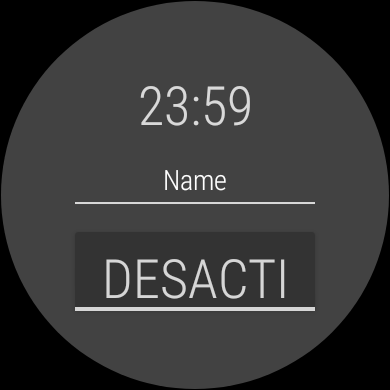
\includegraphics[width=\linewidth]{appActivity.png}
      \caption{Aplicación de gestión}
      \label{fig:uiActivity}
  \end{subfigure}
  \hfill
  \begin{subfigure}[b]{}
      \centering
      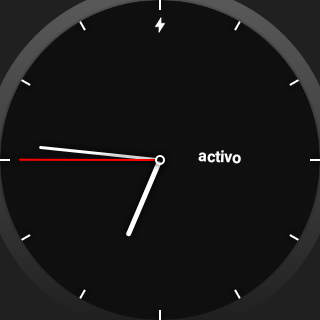
\includegraphics[width=\linewidth]{appWatchface.png}
      \caption{\textit{Watchface}}
      \label{fig:uiWatchface}
  \end{subfigure}
\fi
\subfloat{\label{fig:uiActivity} Aplicación de gestión}{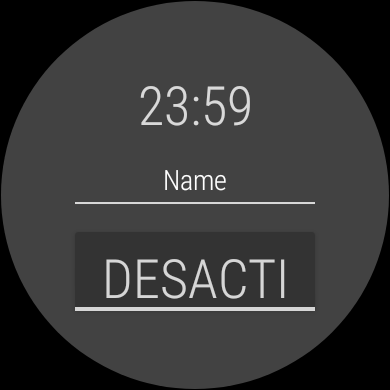
\includegraphics[width=0.4\linewidth]{appActivity.png}}
     \caption{\label{fig:uiApps} Interfaces de usuario}
     \hfill
\subfloat{\label{fig:uiWatchface} Watchface}{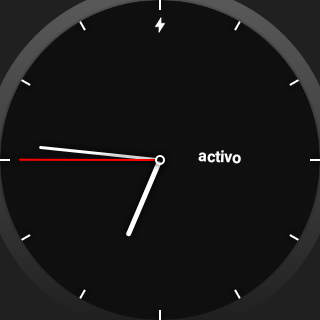
\includegraphics[width=0.4\linewidth]{appWatchface.png}}

\end{figure}



\end{document}

